\chapter{$ISA^{2}$}

Hemos hablado en la introducción sobre las soluciones \ac{ISA} a grandes rasgos y la principal novedad de $ISA^{2}$ frente a éstas. En este capítulo vamos a comenzar revisando el estado del arte (Sección \ref{sec:isa2_estado_del_arte}, destacando trabajos relacionados en el ámbito de las soluciones \ac{ISA}. En la Sección \ref{sec:isa2_model}, detallaremos el sistema $ISA^{2}$ sobre el que hemos trabajado en este proyecto. Finalmente, la Sección \ref{sec:isa2_modelo_nuevo} incluye la descripción de los cambios que hemos implementado sobre el sistema original para hacerlo más rápido y eficaz.


\section{Trabajos relacionados}
\label{sec:isa2_estado_del_arte}

Existen soluciones comerciales para \ac{ISA} como SpeedAlert \cite{soluciones_comerciales} y SpeedShield basadas en tecnología GPS proporcionando información vial (como límites de velocidad y velocidad del vehículo) y regulando la velocidad según ésta \cite{speedshield}.

Actualmente, con la ayuda de una cámara frontal, estos sistemas son capaces de reconocer las señales de tráfico y trabajar en conjunto con una base de datos de límites de velocidad por GPS para mantener la velocidad adecuada en cada tramo \cite{sol_img}.

Sin embargo, ninguna de éstas quieren afrontar el problema estimando la velocidad.

Lo más aproximado a nuestros intereses son una serie de trabajos que estiman la velocidad en vehículos con una secuencia de vídeos grabados por una cámara de vigilancia \cite{isa2} \cite{shukla}. En nuestro caso, la cámara iría en el propio vehículo distinguiendo cada parte del escenario y prediciendo la velocidad en consecuencia.

%TODO_DONE: Añadir una revisión del estado del arte en tecnología ISA. Describir primero soluciones comerciales, y cómo funcionan. Luego añadir otro párrafo de soluciones que se basen en imágenes o que sean papers que soluiones el problema. Puedes traducir y reescibir de nuevo la sección del estado del arte del paper de ISA^2.

\section{El modelo $ISA^{2}$}
\label{sec:isa2_model}

En esta sección vamos a describir cómo funciona todo el sistema $ISA^{2}$, centrándonos en cada parte que lo compone para que resulte más fácil su comprensión. He aquí unas figuras ilustrativas que nos servirán como punto de referencia durante todo el capítulo.


\begin{figure}[H]
  \centering
  \includegraphics[width=8cm]{Figuras/Figura_Esquema_ISA2_Version_1_SegSem.eps}
  \caption{Esquema $ISA^{2}$ Antiguo}
  \label{fig:Isa_v1}
\end{figure}

Como se puede ver al pie de la figura \ref{fig:Isa_v1}, este fue el esquema utilizado para la primera versión de $ISA^{2}$, publicada en \cite{isa2}, cuyo funcionamiento pasamos a detallar.
%TODO_DONE: No lo hagas con item, hay que hacerlo con párrafos extensos, donde puedas resumir todo el artículo del ISA^2. Ya te anticipo que faltan bastantes detalles. El TFG no es un diario de trabajo, es un documento técnico, donde debes demostrar soltura, y reflejar los conocimientos que has aprendido.


En primera instancia el sistema recogía un set de imágenes que se correspondía con situaciones de tráfico, tanto en autovía (o autopista) como en núcleos urbanos. En concreto, la base de datos que se ofrece en \cite{isa2} consistía en dos carpetas: ``\textbf{Highway}'' y ``\textbf{Urban}'', que se correspondían con secuencias de imágenes de autovías y núcleos urbanos respectivamente. En cada una de ellas había una serie de subcarpetas en las que se almacenaban dichas secuencias; para \textbf{Highway} había dos (\textbf{H1} y \textbf{H2}) y para \textbf{Urban} tres (\textbf{U1}, \textbf{U2} y \textbf{U3}).

En ambas carpetas había \textbf{10417} imágenes en total (\textbf{4962} en Highway y \textbf{5455} en Urban).

En la siguiente figura se puede ver un ejemplo del contenido de las mismas:

\begin{figure}[H]
  \centering
  \begin{subfigure}[b]{0.45\linewidth}
    \includegraphics[width=\linewidth]{Figuras/Ejemplo_Highway.eps}
    \caption{Highway}
  \end{subfigure}
    \begin{subfigure}[b]{0.45\linewidth}
    \includegraphics[width=\linewidth]{Figuras/Ejemplo_Urban.eps}
    \caption{Urban}
  \end{subfigure}
  \caption{Imágenes de $ISA^{2}$}
  \label{fig:HyU}
\end{figure}

%TODO_DONE: añade detalles de las secuencias, número de imágenes, figura con las mismas, etc.

Para cada imagen de la base de datos se dispone de la anotación de la velocidad a la que el vehículo debe de circular. Este proceso de anotación se hizo dándo indicaciones a los conductores que participaron de la adquisición de las secuencias de vídeo mientras conducían. Así pues, se dispone de una base de datos con imágenes y velocidades asociadas, que se empleó para entrenar soluciones de inteligencia artificial y visión computador, que fuesen capaces de realizar una regresión, para una imagen de entrada, de la velocidad a la que debía circular el vehículo. A continuación pasamos a describir todos los detalles de la implementación presentada en \cite{isa2}.

%TODO_DONE: Empieza a dar más detalles técnicos de todas las partes del sistema. Hay que explicar todo.
El sistema comienza realizando una \ac{SS} de la imagen de entrada. La \ac{SS} es un proceso por el cual los píxeles de una imagen son dotados de distintos valores para poder diferenciarlos en etiquetas unos de otros y así reconocer los elementos que componen dicha imagen \cite{deeplab}. Se hace mediante el uso de modelos de inteligencia artificial configurados y entrenados para la \ac{SS}, usando en su interior herramientas de deep learning como \textbf{PyTorch} \cite{pytorch}, de la que hablaremos más adelante. He aquí un ejemplo para mostrar el resultado del proceso:

\begin{figure}[H]
  \centering
  \begin{subfigure}[b]{0.45\linewidth}
    \includegraphics[width=\linewidth]{Figuras/Imagen_Original.eps}
    \caption{Imagen Original}
    \label{fig:ImgOrig}
  \end{subfigure}
    \begin{subfigure}[b]{0.5\linewidth}
    \includegraphics[width=\linewidth]{Figuras/Ejemplo_Imagen_Segmentada.eps}
    \caption{Imagen Segmentada}
    \label{fig:ImgSegm}
  \end{subfigure}
  \caption{Ejemplo de \ac{SS}}
  \label{fig:SS}
\end{figure}

%TODO_DONE: añade imagen con segmentación semántica y laimagen sin segmentar, y adaptas el texto de este párrafo que de dejo comentado.
En la figura \ref{fig:SS} se puede ver la imagen de un camión, entre otros elementos, en una autovía (\ref{fig:ImgOrig}). A priori, todos los píxeles de la imagen no están categorizados y no se sabe qué partes de la imagen corresponden al camión, a la carretera, a la señal... Gracias a la segmentación semántica los píxeles de la imagen adquieren los valores de las etiquetas referentes a un \textbf{camión}, una \textbf{carretera} y una \textbf{señal de tráfico} entre otros; y son fácilmente distinguibles entre sí (\ref{fig:ImgSegm}). 

Para la \ac{SS}, el modelo en \cite{isa2} empleó la arquitectura conocida como \textbf{DeepLab} \cite{deeplab}. \textbf{DeepLab} necesita recibir como entrada la imagen en diferentes escalas. Este modelo tenía como base una \ac{CNN}, es decir, una \textbf{Red Neuronal Convolucional} \cite{cnn}, llamada \textbf{ResNet-101} \cite{resnet}.

Para la primera de versión de $ISA^{2}$ \cite{isa2}, DeepLab se entrenó con imágenes en diferentes escalas como entrada, usando factores de escalado de \textbf{0.5}, \textbf{0.75} y \textbf{1}. Más adelante se fusionaban las predicciones de la segmentación para cada escala, cogiendo la mejor respuesta dada por la red en cada escala. Puesto que la base de datos de $ISA^{2}$ no tenía máscaras de segmentación (anotaciones de \ac{SS} para poder compararlas con las predicciones), DeepLab se entrenó sobre la base de datos de \textbf{Cityscapes} \cite{cityscapes}.
%TODO_DONE: falta una breve descripción del modelo. Un párrafo es suficiente.
 

%TODO_DONE: Falta convertir estos item en párrafos como yo he hecho con el primero. Hay que explicar cada paso en detalle: los histogramas, las pirámides (qué son?, niveles?, cómo se computan?), los modelos de regresión que se probaron, etc.

Tras este proceso, mediante unos códigos de \textbf{Matlab} se recogían los datos de los píxeles ya segmentados y se organizaban en histogramas para cada imagen. Estos histogramas se organizaban según la subcarpeta de imágenes correspondiente (\textbf{H1} y \textbf{H2} para Highway y \textbf{U1}, \textbf{U2} y \textbf{U3} para Urban) para mostrar el porcentaje de píxeles referentes a una etiqueta en una determinada imagen. Basándonos en los histogramas generados, usábamos una estrategia llamada \ac{SPP} \cite{spp} para crear un descriptor de imagen por cada histograma.

\begin{figure}[H]
\centering
\includegraphics[width=12cm]{Figuras/SPP.eps}
\caption{\ac{SPP}}
\label{fig:spp}
\end{figure}

Como se puede ver en la figura \ref{fig:spp}, \ac{SPP} (también conocida como ``multi-level pooling'') es una técnica usada para que cualquier imagen, en cualquier escala, pueda ser procesada correctamente por una \ac{CNN}. Consiste en la agrupación de distintas imágenes de entrada procesadas, con diferente escalado, para obtener una salida uniforme. Existen \ac{CNN}s que requieren de una escala fija para una imagen de entrada para un procesamiento óptimo, por lo que se limita la precisión de la predicción. Aplicando \ac{SPP} al final de una \ac{CNN} esta limitación desaparece.


Para ello, y siguiendo la figura \ref{fig:spp}, \ac{SPP} recoge los mapas de características (de un tamaño cualquiera y provenientes de las imágenes de entrada) procesados por las capas convolucionales previas a ésta, y los divide en un número de ``compartimentos espaciales'' con un tamaño proporcional al de la imagen \cite{spp2}. Estos compartimentos vendrán dados con diferente granularidad, es decir, con diferentes niveles de detalle. Dependiendo del nivel de agrupación que se quiera usar habrá un mayor o menor nivel de granularidad y, por ende, habrá mayor o menor información para el descriptor de imagen.


Una vez conseguíamos el descriptor generado en el paso anterior, éste se pasaba a diferentes sistemas de regresión (programados en MatLab): \textbf{Lineal}, \textbf{Lasso}, \textbf{Boosting Trees} y \ac{SVR}, de los cuales hablaremos más adelante. Para cada uno de ellos se añadía \ac{SI} (nivel de granularidad) usando \ac{SPP} de hasta 3 niveles de agrupación para poder compararlos entre sí y saber cuál era mejor (\cite{isa2}). Para ello cogíamos los mejores resultados de cada sistema entre todos los niveles usados, y los usábamos como referencia del sistema.

%TODO_DONE: toda esta subsección hay que moverla al capítulo de resultados, donde explicas la métrica

\section{Propuesta de modelo $ISA^{2}$ mejorado}
\label{sec:isa2_modelo_nuevo}
El trabajo fundamental de este TFG ha consistido en mejorar el sistema tradicional $ISA^{2}$. Nuestro objetivo con este TFG es el de conseguir un sistema $ISA^{2}$ que pueda funcionar en tiempo real, y que consuma pocos recursos de GPU, para poder ser embebido en una plataforma de procesado dentro de un vehículo inteligente. La solución descrita en \cite{isa2} no cumplía ninguno de estos requisitos, principalmente por el sistema DeepLab que llevaba integrada. DeepLab es un modelo que da excelentes prestaciones en cuanto a segmentación semántica se refiere, pero no funciona en tiempo real, y además necesita una tarjeta de procesado con mucha memoria de GPU y muy alto consumo.

Los modelos en tiempo real tienen, como principal objetivo, cumplir con los resultados de un modelo basado en \ac{DCNN} como DeepLab, ya que éstos son los que mejores prestaciones suelen dar debido a los recursos computacionales tan potentes que usan, sin los inconvenientes que ellos mismos traen consigo. Modelos como ERFNet \cite{erfnet} o ICNet \cite{icnet} lo consiguen usando arquitecturas más ligeras en comparación (aunque no sean las adecuadas el reconocimiento de imágenes a gran escala).

Uno de los inconvenientes más importantes de los modelos en tiempo real es el campo de visión \cite{swiftnet}. El campo de visión es realmente grande cuando se trabaja con modelos como DeepLab porque su arquitectura puede soportar tales cantidades de información mientras que en los modelos en tiempo real, éste se reduce. Es por ello que actualmente se tratan con técnicas como \textbf{pirámides de resolución} (\textit{resolution pyramids}) o \textbf{conexiones laterales} (\textit{lateral connections}) para compensarlo.

Por otro lado, la principal ventaja (y la más evidente) de estos modelos es el bajo consumo de GPU en comparación, además del uso de arquitecturas mucho más ligeras que en la otra clase de modelos. Esto hace posible el procesado de imágenes sea más rápido y, por lo tanto, la toma de decisiones también.

Como ya hemos dicho lo ideal sería encontrar un modelo en tiempo real que pueda detectar los objetos de las imágenes con una precisión exquisita, y con un bajo consumo de la GPU, y poco a poco se está consiguiendo.
%TODO_DONE: Sigue motivanto tú el trabajo, saca información del artículo siftwnet. en la intro se ve que hay familias de modelos que funcionan en real-time, ventajas, inconvenientes.


En resumen, para conseguir un modelo $ISA^{2}$ más rápido y eficaz, hemos decidido cambiar el sistema de segmentación semántica Deeplab por el conocido como \textbf{Swiftnet} \cite{swiftnet}. La idea puede verse reflejada en la Figura \ref{fig:Isa_v2}.

\begin{figure}[H]
  \centering
  \includegraphics[width=8cm]{Figuras/Figura_Esquema_ISA2_Version_2.eps}
  \caption{Esquema $ISA^{2}$ Actual}
    \label{fig:Isa_v2}
\end{figure}


Como se puede comprobar, el esquema de la figura \ref{fig:Isa_v2} sigue el mismo camino que el de la primera versión, salvo por unas modificaciones al principio que pasamos a explicar a continuación:

\begin{enumerate}

\item Las imágenes de entrada al modelo de \ac{SS} no llegan en diferentes escalas como se podría intuir. La razón de por qué es así es Swiftnet: El modelo admite tanto imágenes en diferentes escalas como imágenes con una única escala. Sin embargo, para este proyecto hemos optado por la recomendación de los autores \cite{github_swiftnet} y hemos decidido hacerlo con una única escala. De esta manera hemos obtenido los resultados esperados con la base de datos de \textbf{Cityscapes} \cite{cityscapes} que ellos mismos utilizaron \cite{swiftnet}.

\item La segunda, y última, modificación es la más obvia: la sustitución del modelo de DeepLab \cite{deeplab} por el modelo de Swiftnet \cite{swiftnet}. A diferencia del primero, Swiftnet es un modelo que opera en tiempo real (\textbf{Real-Time}) de tal modo que cuando procesa una imagen lo hace en el momento, a una tasa de 39.9 \ac{FPS} \cite{swiftnet}. %TODO_DONE: añade la velocidad a la que funciona en frames por segundo, seguro que viene en el paper original de siftnet.

\end{enumerate}


En el siguiente capítulo hablaremos acerca de la implementación de Swiftnet y de cómo es mejor para los campos de aplicación, especificados anteriormente, con respecto a DeepLab.
